\documentclass[11pt,a4paper]{article}
\usepackage[utf8]{inputenc}
\usepackage[T1]{fontenc}
\usepackage{amsfonts}
\usepackage[french]{babel}
\frenchbsetup{StandardLists=true}
\usepackage{enumitem}
\usepackage{amssymb}
\usepackage{amsmath}
\usepackage{parskip}
\usepackage[left=2cm,right=2cm,top=2cm,bottom=2cm]{geometry}
\usepackage{multirow}
\usepackage[dvipsnames]{xcolor}

\usepackage[T1]{fontenc}
\usepackage{fouriernc}
\usepackage{graphicx}

\usepackage{setspace}
\singlespacing

\usepackage{pstricks}
\usepackage{xkeyval}
\usepackage{pst-labo}

\usepackage{multicol}
\usepackage{caption}
\usepackage{fancyhdr}
\pagestyle{fancy}
\renewcommand\headrulewidth{1pt}
\fancyhead[L]{Lycée Denis Diderot }
\fancyhead[R]{Classe de 1 Bac Pro }
\setcounter{page}{9}\fancyfoot[C]{page \thepage}
\fancyfoot[R]{Année 2024-2025}
\fancyfoot[L]{Alexis RUIZ}
\usepackage{multirow,tabularx,booktabs}
\newcommand{\cadreblanc}[1]{%
\medskip\framebox[\linewidth][c]{%
\rule{0mm}{#1mm}}\par
\medskip}

\usepackage{eurosym}
\usepackage{awesomebox}
\setlength{\aweboxvskip}{0mm}
\usepackage{pifont}
\usepackage{chemmacros}
\usepackage{chemist}
\chemsetup{modules=all}
\usepackage{colortbl}

\renewcommand{\arraystretch}{2.5}
\newcolumntype{C}[1]{>{\centering\arraybackslash }b{#1}}
\newcommand*\acocher{\quitvmode{\fboxsep0pt \fboxrule0.8pt \fbox{\vrule height1.8ex depth.1ex width0pt \vrule height0pt depth0pt width1.9ex }}}

% Commande réponse
\newcommand{\reponse}[1]{%
\fcolorbox{red}{white}{%
\begin{minipage}{\linewidth-2\fboxsep-2\fboxrule}
\textcolor{red}{#1}
\end{minipage}}}


\begin{document}

\begin{center}
\LARGE{\textcolor{red}{\textbf{CORRIGÉ}} — Évaluation - Pression et forces pressantes}\\[8mm]
\end{center}
\normalsize
\hrule

\vspace{8mm}

%%%%%%%%%%%%%%%%%%%%%%%%%%%%%%%%%%
%           EXERCICE 1           %
%%%%%%%%%%%%%%%%%%%%%%%%%%%%%%%%%%

\noindent\fbox{\textbf{Exercice 1 : Choisir la (ou les) bonne(s) réponse(s)}} \hfill \textbf{5 pts}

\begin{tabular}{p{2mm} p{5.5cm}|C{3cm}|C{3cm}|C{3cm}}

    \ding{202} & La pression peut s'exprimer en :& \textcolor{red}{$\boxtimes$ ~~Pascal (Pa)} & \textcolor{red}{$\boxtimes$ ~~Atmosphère (atm)}   & $\Box $ ~~Watt (W) \\
     \hline
  \ding{203} & On mesure la pression atmosphérique à l'aide   & $\Box $ ~~d'un manomètre & $\Box $ ~~d'un thermomètre  & \textcolor{red}{$\boxtimes$ ~~ d'un baromètre} \\
    \hline
     \ding{204} & Avec la formule $P=\dfrac{F}{S}$, on obtient S avec  &$\Box $ ~~ $S=P \times F$  &$\Box $ ~~ $S=\dfrac{P}{F}$  & \textcolor{red}{$\boxtimes$ ~~$S=\dfrac{F}{P}$}   \\
     \hline
     \ding{205} & Dans l'eau, la pression augmente de 1 bar tous les 10m de profondeur, à 120 m (record du monde)  elle est   &$\Box $ ~~ 120 bar &$\Box $ ~~ 12 bar & \textcolor{red}{$\boxtimes$ ~~13,013 bar} \\
     \hline
    \ding{206} & Quand on utilise la loi de Mariotte, à température constante,  si la pression, $p$, est multipliée par 5 alors &$\Box $ ~~ le volume V est inchangé &$\Box $ ~~ le volume V est multiplié par 5  & \textcolor{red}{$\boxtimes$ ~~ le volume V est divisé par 5}  \\

     \end{tabular}

\vspace{3mm}

%%%%%%%%%%%%%%%%%%%%%%%%%%%%%%%%%%
%           EXERCICE 2           %
%%%%%%%%%%%%%%%%%%%%%%%%%%%%%%%%%%

\noindent\fbox{\textbf{Exercice 2 - compléter le tableau suivant : }} \hfill \textbf{3 pts}

\begin{center}
    \renewcommand{\arraystretch}{3}
    \begin{tabular}{|p{6cm}|C{3cm}|C{3cm}|C{3cm}|}
         \hline
      & $P$ & $F$ & $S$ \\
         \hline
         \ding{202} \newline \textcolor{red}{Forme : $F = p \times S$} &  1,013 bar \newline $= 1{,}013 \times 10^5$~Pa  & \textcolor{red}{$\approx 1{,}52 \times 10^5$~N} & 1,5 $m^2$\\
         \hline
         \ding{203} \newline \textcolor{red}{Forme : $p = \dfrac{F}{S}$} & \textcolor{red}{$\approx 1{,}2 \times 10^5$~Pa} & 55 N & 4,5 $cm^2$ \\
         \hline
         \ding{204} \newline \textcolor{red}{Forme : $S = \dfrac{F}{p}$} & $3 \times 10^5$~Pa & 15 N & \textcolor{red}{$5 \times 10^{-5}$~m$^2$}\\
         \hline
    \end{tabular}
\end{center}

\vfill

\newpage

%%%%%%%%%%%%%%%%%%%%%%%%%%%%%%%%%%
%           EXERCICE 3           %
%%%%%%%%%%%%%%%%%%%%%%%%%%%%%%%%%%

\noindent\fbox{\textbf{Exercice 3}} \hfill \textbf{4 pts}

\vspace{1mm}

\noindent%
\begin{minipage}{.36\textwidth}%
Un alpiniste emporte avec lui une bouteille de 2L, fermée hermétiquement au niveau de la mer. Il monte au sommet de l'Everest où la pression atmosphérique n'est plus que de 34 kPa. \\
En supposant que les parois de la bouteille sont extensibles, calculer, en L, le volume de la bouteille au sommet de l'Everest.

\end{minipage}%
\hfill
\begin{minipage}{.55\textwidth}%
\reponse{
\textbf{Données :}\\
$p_1 = 1$ atm $= 101\,300$~Pa $= 101{,}3$~kPa \quad $V_1 = 2$~L\\
$p_2 = 34$~kPa $= 34\,000$~Pa\\[2mm]
\textbf{Loi de Boyle-Mariotte :} $p_1 \times V_1 = p_2 \times V_2$\\[1mm]
$V_2 = \dfrac{p_1 \times V_1}{p_2} = \dfrac{101\,300 \times 2}{34\,000}$\\[3mm]
\[\boxed{V_2 \approx 5{,}96 \text{ L} \approx 6 \text{ L}}\]
\vspace{1mm}
}
\end{minipage}%

\vfill

%%%%%%%%%%%%%%%%%%%%%%%%%%%%%%%%%%
%           EXERCICE 4           %
%%%%%%%%%%%%%%%%%%%%%%%%%%%%%%%%%%

\noindent\fbox{\textbf{Exercice 4 - Pression et force pressante}} \hfill \textbf{3 pts}

\vspace{2mm}

Un bloc de béton de masse $m = 500$~kg est posé à plat sur le sol. La surface de contact avec le sol est de $S = 0{,}25$~m$^2$. On prendra $g = 9{,}81$~N/kg.

\begin{enumerate}

    \item À l'aide de la formule $F = m \times g$, calculer la valeur de $F$ en Newton (N).

    \reponse{
    $F = m \times g = 500 \times 9{,}81$\\[2mm]
    \[\boxed{F = 4\,905 \text{ N}}\]
    \vspace{1mm}
    }

    \item À l'aide de la relation $p = \dfrac{F}{S}$, calculer la pression $p$ exercée par le bloc sur le sol, en Pascal (Pa).

    \reponse{
    $p = \dfrac{F}{S} = \dfrac{4\,905}{0{,}25}$\\[2mm]
    \[\boxed{p = 19\,620 \text{ Pa}}\]
    \vspace{1mm}
    }

    \item Convertir cette pression en bar. \textit{(Rappel : 1 bar = $10^5$ Pa)}

    \reponse{
    $p = \dfrac{19\,620}{10^5}$\\[2mm]
    \[\boxed{p \approx 0{,}20 \text{ bar}}\]
    \vspace{1mm}
    }

\end{enumerate}

\vfill

\newpage

%%%%%%%%%%%%%%%%%%%%%%%%%%%%%%%%%%
%           EXERCICE 5           %
%%%%%%%%%%%%%%%%%%%%%%%%%%%%%%%%%%

\noindent\fbox{\textbf{Exercice 5}} \hfill \textbf{5 pts}
\begin{center}
\textbf{Comment soulever une charge lourde ? }
\end{center}

\noindent%
\begin{minipage}{.70\textwidth}%
Dans l'industrie, un palonnier à ventouses permet la manipulation de charges lourdes à l'aide de ventouses.
\end{minipage}%
\hfill
\begin{minipage}{.25\textwidth}%
\fbox{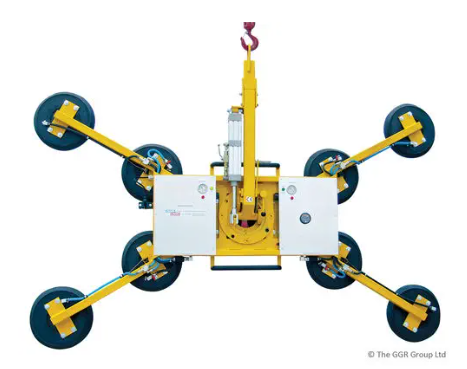
\includegraphics[width=\textwidth]{images/exo4.png}}
\end{minipage}%

\textbf{\ding{202} S'approprier} \\

Lorsqu'une ventouse est simplement posée sur le sol que pouvez vous dire de la pression de l'air au-dessus de la ventouse ? \\

\reponse{La pression au-dessus de la ventouse est égale à la \textbf{pression atmosphérique} $p_{atm} = 1$~bar, car la ventouse est simplement posée et l'air est en contact libre avec l'extérieur.}

\vspace{3mm}

\textbf{\ding{203} Analyser - Raisonner} \\
\begin{enumerate}

\item Que se passe-t-il lorsque l'on appuie sur la ventouse ?

\reponse{En appuyant sur la ventouse, on \textbf{chasse l'air} présent sous la ventouse. La pression sous la ventouse \textbf{diminue} par rapport à la pression atmosphérique.}

\item D'après la loi de Mariotte, comment varient le volume et la pression sous la ventouse lorsqu'on la comprime ?

\reponse{D'après la loi de Boyle-Mariotte ($p \times V = \text{cste}$), quand on comprime la ventouse, le \textbf{volume diminue}, donc la \textbf{pression augmente} momentanément ce qui force l'air à s'échapper. Une fois collée à la surface, il reste une pression $p_v < p_{atm}$ sous la ventouse.}

\end{enumerate}

\vspace{3mm}

\textbf{\ding{204} Réaliser} \\[3mm]

\begin{enumerate}

\noindent%
\begin{minipage}{.56\textwidth}%

  \item La force de préhension est donnée par : \Large{$$F=(p_{atm}-p_v)\times S$$}

\end{minipage}%
\hfill
\begin{minipage}{.35\textwidth}%
 avec : $p_{atm}$~pression atmosphérique ;\\ $p_v$~pression sous la ventouse \\ $S$~surface de contact de la ventouse.
\end{minipage}%
\vspace{3mm}

Calculer, en Newton (N), la valeur  $F$ de la force de préhension sachant que $S = 0{,}08$~m$^2$, $p_v= 0{,}5 \times 10^5$~Pa et $p_{atm}= 1 \times 10^5$~Pa. Arrondir à l'unité.

\reponse{
$F = (p_{atm} - p_v) \times S = (1 - 0{,}5) \times 10^5 \times 0{,}08 = 0{,}5 \times 10^5 \times 0{,}08$\\[2mm]
\[\boxed{F = 4\,000 \text{ N}}\]
\vspace{1mm}
}

\newpage

\item Le palonnier étant équipé de quatre ventouses, calculer, en Newton (N), la valeur total $F_t$ de la force exercée sur l'objet à manipuler.

\reponse{$F_t = 4 \times F = 4 \times 4\,000$\\[2mm] \[\boxed{F_t = 16\,000 \text{ N}}\] \vspace{1mm}}

\item Cette valeur, $F_T$, équivaut à une masse à soulever avec la formule $m=\dfrac{F_T}{9{,}81}$ avec la force en Newton (N) et la masse en kilogramme (kg).

Calculer, en kg, la masse correspondante.

\reponse{$m = \dfrac{F_T}{9{,}81} = \dfrac{16\,000}{9{,}81}$\\[2mm] \[\boxed{m \approx 1\,631 \text{ kg}}\] \vspace{1mm}}

\end{enumerate}

\ding{205} Valider

Le panneau de 1,2 tonne pourra-t-il être soulevé en toute sécurité ?

\reponse{$m_{max} = 1\,631$~kg $> 1\,200$~kg (1,2~tonne). Le palonnier peut exercer une force suffisante pour soulever le panneau. \textbf{Oui, il pourra être soulevé en toute sécurité.}}

\vspace{3mm}

\ding{206} Communiquer

Expliquer en quelques lignes le fonctionnement d'un palonnier à ventouses.

\reponse{En comprimant les ventouses contre la surface de l'objet, on expulse l'air sous celles-ci, créant une \textbf{dépression} (pression $p_v < p_{atm}$). La pression atmosphérique s'exerce alors sur la face supérieure des ventouses et crée une \textbf{force de préhension} plaquant l'objet contre le palonnier. Cette force permet de soulever des charges lourdes.}

\vfill

%%%%%%%%%%%%%%%%%%%%%%%%%%%%%%%%%%
%           ÉNIGME BONUS         %
%%%%%%%%%%%%%%%%%%%%%%%%%%%%%%%%%%

\begin{center}
\fcolorbox{black}{black!5}{%
\begin{minipage}{0.95\linewidth}
\vspace{2mm}
\begin{center}
\large\textbf{\ding{72}~~Question Bonus~~(+1 point)~~\ding{72}}
\end{center}
\vspace{1mm}
\textbf{Énigme :} Si \textbf{5 machines} fabriquent \textbf{5 pièces} en \textbf{5 minutes}, combien de temps faut-il à \textbf{100 machines} pour fabriquer \textbf{100 pièces} ?\\[2mm]
\textbf{Justifier votre réponse.}
\vspace{2mm}
\end{minipage}}
\end{center}

\reponse{
\textbf{Raisonnement :} 5 machines font 5 pièces en 5 minutes $\Rightarrow$ \textbf{1 machine fait 1 pièce en 5 minutes}.\\
Donc 100 machines font 100 pièces en \textbf{5 minutes} (chaque machine produit sa pièce en 5 min, toutes en parallèle).\\[2mm]
\textbf{Le piège :} répondre 100 minutes en divisant 100 par 1 pièce/minute — c'est faux car on raisonne sur 1 machine, pas 100.\\[1mm]
\[\boxed{\text{Réponse : } \textbf{5 minutes}}\]
\vspace{1mm}
}

\vfill

\newpage

%%%%%%%%%%%%%%%%%%%%%%%%%%%%%%%%%%
%       GRILLE DE CORRECTION     %
%%%%%%%%%%%%%%%%%%%%%%%%%%%%%%%%%%

\thispagestyle{empty}

\begin{center}
\large\textbf{GRILLE DE CORRECTION}\\[3mm]
\textbf{Évaluation — Pression et forces pressantes} \hfill \textbf{Total : /20 pts}
\end{center}

\vspace{3mm}

\renewcommand{\arraystretch}{1.8}

\begin{tabular}{|C{1.8cm}|C{1.5cm}|p{8.5cm}|C{1.3cm}|C{1.3cm}|}
\hline
\rowcolor{gray!30}
\textbf{Exercice} & \textbf{Question} & \textbf{Critères de correction} & \textbf{Barème} & \textbf{Note} \\
\hline
\multirow{5}{*}{\textbf{Ex 1} \newline \textit{5 pts}}
& \ding{202} & Pascal (Pa) ET Atmosphère (atm) cochés & 1 pt & \\
\cline{2-5}
& \ding{203} & Un baromètre & 1 pt & \\
\cline{2-5}
& \ding{204} & $S = \dfrac{F}{P}$ & 1 pt & \\
\cline{2-5}
& \ding{205} & 13,013 bar & 1 pt & \\
\cline{2-5}
& \ding{206} & Le volume V est divisé par 5 & 1 pt & \\
\hline
\multirow{3}{*}{\textbf{Ex 2} \newline \textit{3 pts}}
& \ding{202} & Forme $F=p\times S$ correcte (0,5 pt) + $F \approx 1{,}52\times10^5$~N avec unité (0,5 pt) & 1 pt & \\
\cline{2-5}
& \ding{203} & Forme $p=F/S$ correcte (0,5 pt) + $p \approx 1{,}2\times10^5$~Pa avec unité (0,5 pt) & 1 pt & \\
\cline{2-5}
& \ding{204} & Forme $S=F/p$ correcte (0,5 pt) + $S = 5\times10^{-5}$~m$^2$ avec unité (0,5 pt) & 1 pt & \\
\hline
\multirow{3}{*}{\textbf{Ex 3} \newline \textit{4 pts}}
& & Identification correcte de $p_1$ et $p_2$ & 1 pt & \\
\cline{2-5}
& & Écriture de la loi de Boyle-Mariotte & 1 pt & \\
\cline{2-5}
& & Calcul de $V_2$ correct avec unité & 2 pts & \\
\hline
\multirow{3}{*}{\textbf{Ex 4} \newline \textit{3 pts}}
& Q1 & $F = m \times g = 4\,905$~N & 1 pt & \\
\cline{2-5}
& Q2 & $p = F/S = 19\,620$~Pa & 1 pt & \\
\cline{2-5}
& Q3 & Conversion $p \approx 0{,}20$~bar & 1 pt & \\
\hline
\multirow{6}{*}{\textbf{Ex 5} \newline \textit{5 pts}}
& \ding{202} & Pression au-dessus = $p_{atm}$ & 0,5 pt & \\
\cline{2-5}
& \ding{203} Q1 & L'air est chassé, la pression diminue sous la ventouse & 0,5 pt & \\
\cline{2-5}
& \ding{203} Q2 & Volume diminue $\Rightarrow$ pression augmente (Boyle-Mariotte) & 0,5 pt & \\
\cline{2-5}
& \ding{204} Q1 & $F = (p_{atm}-p_v)\times S = 4\,000$~N & 1,5 pt & \\
\cline{2-5}
& \ding{204} Q2+Q3 & $F_t = 16\,000$~N et $m \approx 1\,631$~kg & 1 pt & \\
\cline{2-5}
& \ding{205}+\ding{206} & Validation correcte + explication cohérente & 1 pt & \\
\hline
\multirow{2}{*}{\textbf{Bonus} \newline \textit{+1 pt}}
& & Réponse correcte (5 minutes) avec justification & 1 pt & \\
\cline{2-5}
& & & & \\
\hline
\rowcolor{gray!20}
\multicolumn{4}{|r|}{\textbf{TOTAL}} & \textbf{/20} \\
\hline
\end{tabular}

\vspace{6mm}

\begin{tabular}{|p{5cm}|p{5cm}|p{5cm}|}
\hline
\textbf{NOM :} & \textbf{Prénom :} & \textbf{Classe :} \\[6mm]
\hline
\multicolumn{2}{|l|}{\textbf{Note :} \hspace{2cm}/20} & \textbf{Appréciation :} \\[6mm]
\hline
\end{tabular}

\end{document}
